\documentclass[10pt]{article}
\usepackage[letterpaper,margin=0.76in]{geometry}
\usepackage[T1]{fontenc}
\usepackage{lmodern}
\usepackage{microtype}
\usepackage{amsmath,amssymb,mathtools}
\usepackage{booktabs}
\usepackage{array}
\usepackage{graphicx}
\usepackage{xcolor}
\usepackage{titlesec}
\usepackage[font=small,labelfont=bf,skip=4pt,hypcap=false]{caption}
\usepackage[numbers,sort&compress]{natbib}
\usepackage[most]{tcolorbox}
\usepackage{enumitem}
\usepackage{hyperref}

\definecolor{ink}{HTML}{000000}
\definecolor{muted}{HTML}{000000}
\definecolor{accent}{HTML}{000000}
\definecolor{boxbg}{HTML}{F2F5F7}
\hypersetup{colorlinks=true,linkcolor=accent,urlcolor=accent,citecolor=accent}
\color{ink}

\titleformat{\section}{\large\bfseries\color{accent}}{}{0pt}{}
\titlespacing*{\section}{0pt}{0.75em}{0.25em}
\setlength{\parindent}{0pt}
\setlength{\parskip}{0.40em}
\setlength{\bibsep}{1pt}
\renewcommand{\bibfont}{\footnotesize}

% --- Conceptual Persuasions callout -------------------------------------
\newtcolorbox{cpbox}{
  enhanced, breakable,
  colback=boxbg, colframe=boxbg,
  boxrule=0pt, arc=2.5pt, outer arc=2.5pt,
  left=10pt, right=10pt, top=7pt, bottom=8pt,
  borderline west={2.4pt}{0pt}{accent},
  before skip=0.95em, after skip=0.95em,
}
\newenvironment{persuasions}
  {\begin{cpbox}\small\setlength{\parskip}{0pt}%
   {\footnotesize\bfseries\color{accent}%
    \textls[110]{CONCEPTUAL PERSUASIONS}}\par\vspace{3pt}%
   \begin{itemize}[leftmargin=1.15em,itemsep=2.5pt,topsep=0pt,parsep=0pt,
                   label=\textcolor{accent}{\scriptsize$\blacktriangleright$}]}
  {\end{itemize}\end{cpbox}}

\title{\vspace{-2.3em}\textbf{Invariant Measures on Compatible Classical Histories}}
\author{J. R. Landers}
\date{}

\begin{document}
\maketitle
\vspace{-1.25em}

\begin{abstract}
The compatible-history program requires a measure on complete trajectories
that does not depend on canonical coordinates, temporal slicing, or gauge.
For deterministic classical systems, that measure need not be invented as an
independent product over time.  A physical initial state determines a complete
solution, so invariant measure on reduced phase space induces a history
measure by pushforward through the solution map.  This paper develops that
construction and tests its unresolved invariances.  A continuous compatibility
functional converges under temporal refinement and agrees to
$1.8\times10^{-5}$ bits after a nonlinear canonical transformation of an
anharmonic oscillator.  Reparameterizing the history by linear, quadratic,
and exponential clocks gives a cross-clock spread of $5\times10^{-6}$ bits
when the lapse is included, while naive slice weighting produces a
$0.0814$-bit artifact.  Finally, a parametrized oscillator with Hamiltonian
constraint is evaluated on two nonlinear gauge surfaces.  The gauge-fixed
Faddeev--Popov measure reproduces the reduced phase volume within $0.0029\%$
and the survival information within $3.6\times10^{-5}$ bits; omitting the
determinant creates false shifts as large as $0.254$ bits.  Surviving-volume
information and posterior Kullback--Leibler information are also shown to be
distinct.  The result supplies a finite constrained classical history measure;
its extension to gravity and its proposed relation to cosmological expansion
remain open.
\end{abstract}

\section*{From invariant states to invariant histories}

The preceding paper, \emph{Noether Constraints and the Measure of Compatible
Histories}, replaced coordinate-cell cardinality with Liouville phase volume.
Its numerical tests separated two objects sharply.  Intersecting-cell counts
retained grid shape and canonical coordinates, while Liouville band density
agreed across those choices.  The paper then asked for the analogous invariant
measure on complete constrained histories and for a temporal normalization
that survives refinement.

The apparent difficulty is that a path contains a value at every time.  If
each temporal slice is counted as another independent coordinate, raw history
cardinality diverges as the slicing is refined.  Deterministic dynamics,
however, makes those values dependent.  Once physical initial data and the
dynamical law are fixed, the trajectory is fixed.  The space of solutions is
therefore not an infinite Cartesian product of independently chosen states;
under suitable existence and uniqueness conditions it is another
representation of physical initial-data space.

Let $\Gamma_{\rm phys}$ be the reduced phase space of physical initial data,
after constraints and gauge redundancy have been removed, and let
$\nu_0$ be a normalized measure on it.  For ordinary Hamiltonian mechanics,
one may write
\begin{equation}
d\nu_0(z)=f_0(z)\,d\mu_L(z),
\qquad
\int_{\Gamma_{\rm phys}}d\nu_0=1,
\label{eq:initial-measure}
\end{equation}
where $z$ denotes initial data, $d\mu_L$ is Liouville measure, and $f_0$ is a
specified ensemble density.  Let
\begin{equation}
F:\Gamma_{\rm phys}\longrightarrow\mathcal H,
\qquad z\longmapsto\gamma_z
\label{eq:solution-map}
\end{equation}
be the solution map into the set $\mathcal H$ of complete classical histories.
The induced history measure is the pushforward
\begin{equation}
\boxed{\mu_{\mathcal H}=F_*\nu_0,}
\qquad
\mu_{\mathcal H}(B)=\nu_0(F^{-1}(B))
\label{eq:pushforward}
\end{equation}
for every measurable set of histories $B\subseteq\mathcal H$.

Equation~\eqref{eq:pushforward} is the central construction.  It assigns
history volume without multiplying coordinate volumes at successive times.
Liouville's theorem preserves the underlying phase volume along Hamiltonian
flow, while the solution map records how one physical state is represented as
an entire path \citep{Liouville1838,Arnold1989}.

The construction also makes canonical invariance direct.  Let
$T:\Gamma_{\rm phys}\to\Gamma'_{\rm phys}$ be a canonical transformation,
let $\widehat T$ be its action on histories, and suppose the transformed
solution map satisfies $F'\circ T=\widehat T\circ F$.  Since
$T_*\nu_0$ is the same physical measure in the new coordinates,
\begin{equation}
F'_*T_*\nu_0
=\widehat T_*F_*\nu_0.
\label{eq:canonical-pushforward}
\end{equation}
Thus both descriptions assign the same measure to the same physical history
event.  Coordinate invariance is inherited rather than imposed afterward.

\begin{persuasions}
\item A deterministic history does not contain one independent state per time
slice.  It contains one physical initial condition represented along its orbit.
\item The continuum path measure is therefore induced from reduced phase
space; it is not obtained by counting increasingly many temporal cells.
\item Canonical invariance of the initial measure propagates to history space
through the solution map.
\item The ensemble density $f_0$ remains physical input.  Invariance specifies
how an ensemble transforms, not which cosmological ensemble nature chooses.
\end{persuasions}

\section*{Compatibility as a functional on histories}

Let $Y_{\leq t}$ denote the physical record accumulated through time $t$.
Represent compatibility with that record by a measurable functional
\begin{equation}
0\leq W_t(\gamma)\leq1.
\label{eq:compatibility-functional}
\end{equation}
A hard compatible set $\mathcal H_t$ is recovered with
$W_t=\mathbf1\{\gamma\in\mathcal H_t\}$.  A soft record can instead grade
histories continuously.  The surviving history weight and its information are
\begin{equation}
Z_t=\int_{\mathcal H}W_t(\gamma)\,d\mu_{\mathcal H}(\gamma),
\qquad
C_{\rm surv}(t)=-\log_2 Z_t.
\label{eq:survival-information}
\end{equation}
When $W_{t_2}\leq W_{t_1}$ for $t_2\geq t_1$, the compatible weights form a
filtration and $C_{\rm surv}$ is nondecreasing.  This is the measure-theoretic
analogue of the original nested-neighborhood theorem.

The same compatibility functional defines a posterior history measure,
\begin{equation}
d\mu_t(\gamma)
=\frac{W_t(\gamma)}{Z_t}\,d\mu_{\mathcal H}(\gamma).
\label{eq:posterior-history}
\end{equation}
Its information gain relative to the prior is the Kullback--Leibler divergence
\citep{KullbackLeibler1951},
\begin{align}
C_{\rm KL}(t)
&=\frac{1}{\ln2}
D_{\rm KL}(\mu_t\Vert\mu_{\mathcal H})\nonumber\\
&=C_{\rm surv}(t)
+\int_{\mathcal H}\log_2 W_t(\gamma)\,d\mu_t(\gamma).
\label{eq:kl-information}
\end{align}
Because $W_t\leq1$, the final term is nonpositive and therefore
\begin{equation}
0\leq C_{\rm KL}(t)\leq C_{\rm surv}(t).
\label{eq:information-inequality}
\end{equation}
For a hard indicator, $W_t=1$ on every surviving history and the two quantities
coincide.  For soft compatibility they generally differ.  Moreover, realized
posterior KL information need not be monotone for every observation sequence,
whereas nested surviving volume is monotone by construction.

The numerical tests use the dimensionless soft functional
\begin{equation}
W_T(\gamma)
=\exp\!\left[-\frac{1}{2\sigma^2}
\int_0^T\bigl(x_\gamma(t)-y(t)\bigr)^2dt\right],
\label{eq:soft-functional}
\end{equation}
where $y(t)$ is the stipulated record and $\sigma$ fixes its physical
resolution.  This is a bounded compatibility score, not a claim that a
particular observational noise law has been derived.

For a harmonic record $y(t)=\cos t$, $\sigma=0.35$, and a uniform Liouville
ensemble on $(x_0,p_0)\in[-1.5,1.5]^2$, both information quantities increased
over the tested record, but they were not equal.

\begin{center}
\captionof{table}{Accumulation of surviving-volume and posterior information.
The difference is structural for a soft compatibility functional.}
\label{tab:information-functionals}
\small
\begin{tabular}{rrrr}
\toprule
$T$ & $C_{\rm surv}$ (bits) & $C_{\rm KL}$ (bits) & Difference (bits)\\
\midrule
$0.5$ & $1.558594$ & $0.969143$ & $0.589450$\\
$1.0$ & $2.238907$ & $1.309413$ & $0.929494$\\
$2.0$ & $3.568521$ & $2.319828$ & $1.248693$\\
$3.0$ & $4.195540$ & $2.872346$ & $1.323194$\\
$4.0$ & $4.546205$ & $3.169442$ & $1.376764$\\
\bottomrule
\end{tabular}
\end{center}

\begin{persuasions}
\item ``Remaining volume'' and ``information learned by an observer'' are not
synonyms once compatibility is soft.
\item The original cosmological bridge refers most directly to
$C_{\rm surv}$ because it is the negative logarithm of surviving measure.
\item Posterior KL information is a complementary observer-relative quantity;
it should not be substituted silently for compatible-history volume.
\item A physical application must specify the ensemble, record, and resolution
before either number is calculated.
\end{persuasions}

\section*{Temporal refinement requires the lapse}

Let $t=f(\tau)$ be a monotone reparameterization of the same history and define
the lapse $N(\tau)=dt/d\tau>0$.  Equation~\eqref{eq:soft-functional} becomes
\begin{equation}
W_T(\gamma)
=\exp\!\left[-\frac{1}{2\sigma^2}
\int d\tau\,N(\tau)
\bigl(x_\gamma(f(\tau))-y(f(\tau))\bigr)^2\right].
\label{eq:lapse-functional}
\end{equation}
The lapse is the Jacobian that makes the exponent an integral over physical
time.  Omitting it assigns equal physical weight to unequal clock intervals
and makes the apparent information depend on the reporting parameter.

The harmonic ensemble was evaluated with $320$ midpoint slices using linear,
quadratic, and exponential clocks over the same physical interval $0\leq
t\leq4$.  With the lapse, the cross-clock spread in $C_{\rm surv}$ was
$5.3\times10^{-6}$ bits.  Replacing $N(\tau)d\tau$ by a constant slice weight
produced a $0.081382$-bit spread.

\begin{center}
\captionof{table}{Clock reparameterization of one physical history functional.
The invariant column includes $dt/d\tau$; the naive column weights coordinate
slices equally.}
\label{tab:clock-test}
\small
\begin{tabular}{lrrr}
\toprule
Clock & Invariant $C_{\rm surv}$ & Invariant $C_{\rm KL}$ & Naive $C_{\rm surv}$\\
\midrule
Linear & $4.5460702$ & $3.1690652$ & $4.546070$\\
Quadratic & $4.5460682$ & $3.1690619$ & $4.464688$\\
Exponential & $4.5460649$ & $3.1690584$ & $4.488662$\\
\bottomrule
\end{tabular}
\end{center}

For the quadratic clock, doubling the slice count from $160$ to $320$ changed
$C_{\rm surv}$ by $1.1\times10^{-5}$ bits.  The temporal divergence in raw
path cardinality is therefore not a required feature of deterministic history
measure.  It arises when temporal labels are counted rather than integrated
with their physical measure.

\begin{persuasions}
\item Time reparameterization does not require a preferred density of
coordinate slices.  It requires the invariant element $dt=N\,d\tau$.
\item Refining the numerical clock then improves quadrature instead of adding
new physical alternatives.
\item This resolves temporal normalization for the tested deparameterizable
systems; it does not select a preferred clock in general relativity.
\end{persuasions}

\section*{Nonlinear canonical invariance}

Exact harmonic flow and a linear canonical shear provide a useful first gate,
but they can hide discretization effects.  The stronger test uses
\begin{equation}
H(x,p)=\frac{p^2}{2}+\frac{x^2}{2}+\frac{\lambda x^4}{4},
\qquad \lambda=0.5,
\label{eq:anharmonic-hamiltonian}
\end{equation}
and the nonlinear canonical transformation
\begin{equation}
Q=x,
\qquad P=p+\alpha x^3,
\qquad \alpha=0.2.
\label{eq:nonlinear-shear}
\end{equation}
Since $dQ\wedge dP=dx\wedge dp$, Liouville area is preserved.  The transformed
Hamiltonian is
\begin{equation}
H'(Q,P)=\frac12(P-\alpha Q^3)^2
+\frac{Q^2}{2}+\frac{\lambda Q^4}{4}.
\label{eq:transformed-hamiltonian}
\end{equation}

A scrambled Sobol ensemble of $131{,}072$ initial conditions was drawn from
$[-1.5,1.5]^2$.  The physical and transformed Hamilton equations were
integrated independently with the explicit midpoint method.  The record was
the high-accuracy anharmonic solution from $(x_0,p_0)=(1,0)$, and the
functional was Eq.~\eqref{eq:soft-functional} with $T=4$ and $\sigma=0.35$.
Because a finite-step integrator is not exactly covariant under nonlinear
coordinate changes, agreement is expected only in the refinement limit.

\begin{center}
\captionof{table}{Nonlinear canonical refinement.  The difference between
coordinate descriptions decreases toward zero with the integration step.}
\label{tab:nonlinear-test}
\small
\begin{tabular}{rrrrr}
\toprule
$\Delta t$ & $C_{x,p}$ & $C_{Q,P}$ & $|\Delta C|$ & $C_{{\rm KL},x,p}$\\
\midrule
$0.1000$ & $4.223811$ & $4.225701$ & $0.001890$ & $2.810564$\\
$0.0500$ & $4.214450$ & $4.214817$ & $0.000367$ & $2.802563$\\
$0.0250$ & $4.211163$ & $4.211242$ & $0.000079$ & $2.799688$\\
$0.0125$ & $4.209709$ & $4.209727$ & $0.000018$ & $2.798383$\\
\bottomrule
\end{tabular}
\end{center}

The finest discrepancy is $1.8\times10^{-5}$ bits.  Its decrease under
refinement distinguishes continuum invariance from an accidental identity in
one coordinate implementation (Fig.~\ref{fig:invariance}).

\section*{Constraint reduction and nonlinear gauges}

Canonical invariance is necessary but not sufficient for a constrained
theory.  Gauge-related points are different descriptions of one physical
history and must not be counted as alternatives.  The standard Hamiltonian
treatment represents a constrained system on an extended phase space and
reduces it by first-class constraints and gauge conditions
\citep{Dirac1964,HenneauxTeitelboim1992}.

The test system is the parametrized unit harmonic oscillator.  Its extended
coordinates are $(x,p,t,p_t)$ and its first-class constraint is
\begin{equation}
\mathcal C=p_t+\frac{x^2+p^2}{2}=0.
\label{eq:parametrized-constraint}
\end{equation}
The parameter labeling the orbit is unphysical; physical time $t$ is itself a
phase-space coordinate.  Complete physical histories can be labeled by the
Dirac observables
\begin{equation}
X=x\cos t-p\sin t,
\qquad
P=x\sin t+p\cos t,
\label{eq:dirac-observables}
\end{equation}
which are the position and momentum at $t=0$ and satisfy
$\{X,\mathcal C\}=\{P,\mathcal C\}=0$.

For one admissible gauge condition $\chi=0$, the gauge-fixed representation of
reduced measure is
\begin{equation}
d\mu_{\rm phys}^{(\chi)}
=\delta(\mathcal C)\,\delta(\chi)\,
\left|\{\chi,\mathcal C\}\right|
\,dx\,dp\,dt\,dp_t.
\label{eq:fp-measure}
\end{equation}
The determinant is the finite-dimensional Faddeev--Popov factor
\citep{FaddeevPopov1967}.  It compensates for the angle at which the gauge
surface intersects gauge orbits.  If $W(X,P)$ is gauge invariant and each
orbit intersects the gauge surface once, the normalized ratio
\begin{equation}
Z_\chi
=\frac{\int W(X,P)\,d\mu_{\rm phys}^{(\chi)}}
       {\int d\mu_{\rm phys}^{(\chi)}}
\label{eq:gauge-ratio}
\end{equation}
is independent of $\chi$.  Geometrically, the Faddeev--Popov determinant is
the Jacobian from gauge-surface coordinates to the orbit labels $(X,P)$.

The physical prior was uniform on $(X,P)\in[-1.5,1.5]^2$, with reduced
Liouville area $9$.  Three gauges were compared:
\begin{align}
\chi_0&=t, & |\{\chi_0,\mathcal C\}|&=1,\nonumber\\
\chi_1&=t+0.15xp,
& |\{\chi_1,\mathcal C\}|&=1+0.15(p^2-x^2),\nonumber\\
\chi_2&=t+0.10x^2,
& |\{\chi_2,\mathcal C\}|&=1+0.20xp.
\label{eq:test-gauges}
\end{align}
The coefficients and bounded domain were chosen so both nonlinear determinants
remain positive.  Each orbit therefore crosses each test surface once; the
experiment deliberately avoids Gribov copies.

Independent scrambled Sobol samples were drawn on each nonlinear gauge
surface.  A mask selected the common square in Dirac-observable space, and
Eq.~\eqref{eq:soft-functional} was evaluated from $(X,P)$.  Estimates were
refined from $65{,}536$ to $1{,}048{,}576$ points.

\begin{center}
\captionof{table}{Constrained-history gauge test at $1{,}048{,}576$ samples.
The Faddeev--Popov columns reproduce reduced measure; the last column omits
the determinant as a controlled failure.}
\label{tab:gauge-test}
\small
\begin{tabular}{lrrrr}
\toprule
Gauge & Area & $C_{\rm surv}^{\rm FP}$ & $C_{\rm KL}^{\rm FP}$ & $C_{\rm surv}^{\rm naive}$\\
\midrule
$t=0$ & $9.000000$ & $4.546071$ & $3.169067$ & $4.546071$\\
$t+0.15xp=0$ & $9.000177$ & $4.546080$ & $3.169041$ & $4.291667$\\
$t+0.10x^2=0$ & $9.000260$ & $4.546107$ & $3.169089$ & $4.588782$\\
\bottomrule
\end{tabular}
\end{center}

Across the nonlinear gauges, the maximum Faddeev--Popov-weighted discrepancy
was $3.6\times10^{-5}$ bits for survival information and
$2.6\times10^{-5}$ bits for KL information.  The largest relative error in
reduced area was $0.00289\%$.  Omitting the determinant produced false shifts
of $0.254404$ and $0.042711$ bits.  Gauge redundancy can therefore manufacture
precisely the kind of apparent history information the construction is meant
to exclude.

\begin{figure}[ht]
\centering
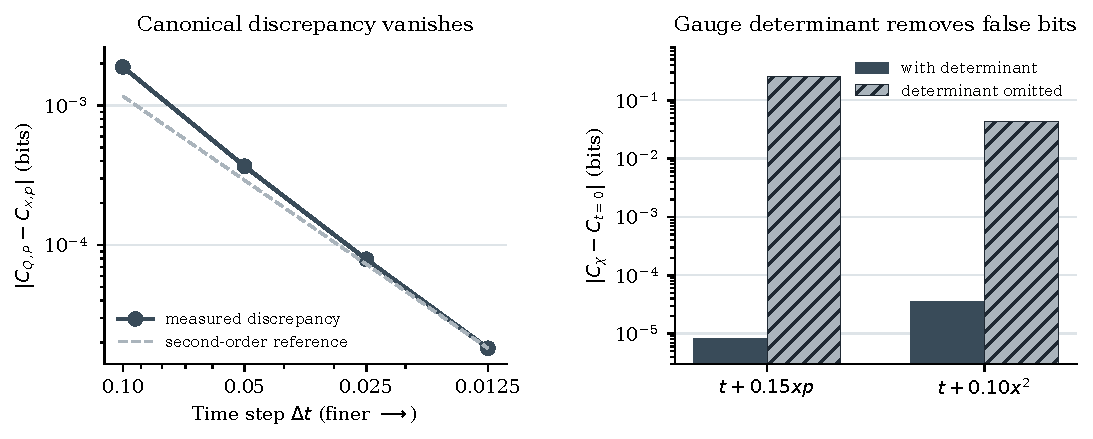
\includegraphics[width=0.98\linewidth]{history_measure_invariance.pdf}
\caption{Two continuum tests separate physical history measure from its
coordinate representation.  Left: independently integrated descriptions of
the anharmonic system converge under a nonlinear canonical transformation.
Right: the gauge-fixed determinant suppresses false information by three to
four orders of magnitude relative to naive gauge-surface weighting.}
\label{fig:invariance}
\end{figure}

\begin{persuasions}
\item A gauge surface is not automatically a uniformly weighted set of
physical alternatives.  Its intersection density with gauge orbits matters.
\item The Faddeev--Popov determinant is not a quantum decoration in this test;
it is the classical Jacobian required to recover reduced Liouville measure.
\item When the determinant is omitted, gauge choice becomes false history
information.  When it is included, both surviving volume and posterior
information recover their reduced-space values.
\item The test excludes local gauge artifacts in a single-constraint system.
It does not address multiple constraints, open gauge algebras, or Gribov
ambiguities.
\end{persuasions}

\section*{The classical history object}

The experiments support one measurement hierarchy for finite deterministic
constrained systems.  Begin with extended phase space, impose the constraints,
quotient gauge redundancy, and normalize a physical ensemble on the resulting
space.  Push that measure through the dynamical solution map.  Finally apply a
gauge-invariant compatibility functional to complete histories:
\begin{equation}
\boxed{
\begin{aligned}
d\mu_{\rm phys}
&\longrightarrow
\mu_{\mathcal H}=F_*\mu_{\rm phys},\\
W_t(\gamma)
&\longrightarrow
Z_t=\int W_t\,d\mu_{\mathcal H},\\
C_{\rm surv}(t)
&=-\log_2 Z_t.
\end{aligned}}
\label{eq:classical-history-object}
\end{equation}
In a gauge-fixed representation, $d\mu_{\rm phys}$ contains the constraints,
gauge conditions, and their determinant as in Eq.~\eqref{eq:fp-measure}.  In a
reduced representation it is simply the symplectic volume on physical degrees
of freedom.  These are two calculations of the same quotient measure.

The construction resolves the temporal-cell problem for this class of
systems.  A complete history is weighted once through its physical initial
data.  Successive observations refine $W_t$; successive numerical slices only
approximate the invariant time integral.  No absolute product of coordinate
cell widths or time steps is required.

The result is classical.  A Lorentzian Feynman integral assigns complex
amplitudes to off-shell paths, not a positive volume on classical solutions.
Quantum probabilities for spacetime alternatives require interference to be
handled, for example through a decoherence functional on coarse-grained
histories \citep{Hartle1993}.  That is a distinct extension rather than a
replacement for Eq.~\eqref{eq:pushforward}.

\section*{What remains open for cosmology}

The accumulated-history proposal relates a three-dimensional relational scale
to surviving history information through
\begin{equation}
H_{\rm rel}(\tau)
=\frac{\ln2}{3}\frac{dC_{\rm surv}}{d\tau}.
\label{eq:cosmological-bridge}
\end{equation}
The present result strengthens the definition of $C_{\rm surv}$ but does not
derive Eq.~\eqref{eq:cosmological-bridge}.  It also does not show that the
history-information rate equals the observed Hubble rate.  The constitutive
identification between inverse compatible-history volume and physical spatial
volume remains a cosmological hypothesis.

Three additional structures are required before that comparison is warranted.
First, general relativity has Hamiltonian and momentum constraints at every
spatial point rather than one deparameterizable constraint.  Its gauge group
includes spacetime diffeomorphisms, and global reduced phase space is difficult
to construct.  Second, observations must be relational and causal: the record
cannot be defined by coordinate time or coordinate position.  Third, the prior
measure on gravitational initial data must be specified independently of the
expansion history it is intended to predict.

The finite result nevertheless changes the next question.  The missing object
is no longer an unrestricted ``measure over every value at every time.''  It
is the reduced symplectic measure on gravitational solution space, together
with a causal relational compatibility functional.  A finite minisuperspace
or constrained cosmological perturbation system is the natural next gate.  It
should be required to pass canonical, clock, gauge, and refinement tests before
any information rate is compared with held-out expansion data.

\begin{persuasions}
\item The invariant classical history measure now has a constructive form:
reduce physical initial data, then push its measure through the dynamics.
\item The lapse removes clock-density artifacts; the gauge determinant removes
orbit-counting artifacts; neither chooses the cosmological ensemble.
\item The Hubble relation remains a constitutive hypothesis.  No cosmological
rate was used to select the measure, gauge, tolerance, or numerical cutoff.
\item Gravity is the next scientific test, while decoherent quantum histories
form a separate later branch.
\end{persuasions}

\section*{Constructive conclusion}
\enlargethispage{2\baselineskip}

The complexity-neighborhoods program began with a combinatorial filtration:
added distinguishing structure removes fixed-radius neighbors.  Its
cosmological development replaced objects by histories, geometric proximity by
conditional dynamical compatibility, and raw state cardinality by invariant
Liouville volume.  The present paper completes the corresponding classical
history step for finite constrained systems.

Physical initial data carry reduced symplectic measure.  Deterministic dynamics
maps those data to complete histories.  Observations weight the histories, the
lapse makes temporal accumulation independent of the clock, and gauge fixing
with its determinant makes the result independent of the representative on an
orbit.  The controlled failures show why every element is necessary: finite
time slices and gauge surfaces can both create false bits when their Jacobians
are ignored.

The resulting object is compact:
\begin{equation}
\boxed{
\text{invariant compatible-history information}
=-\log_2\!\int_{\Gamma_{\rm phys}}
W_t(\gamma_z)\,d\nu_0(z).}
\label{eq:final-object}
\end{equation}
The tested quantity is canonical, clock, and gauge invariant.  Whether a
gravitational analogue flows at the expansion rate remains open.

\bibliographystyle{unsrtnat}
\bibliography{../../references/complexity_cosmology}

\end{document}
